\section{Autoinducer analogue-ciprofloxacin conjugates}

\subsection{Inspiration}

The formation of biofilms can drastically increase MIC for many antibiotics \cite{Ceri1999}. For ciprofloxacin in \textit{P. aeruginosa} the MIC increases by 16 fold according to Ceri et al. 

Ganguly et al. \cite{Ganguly2011} found the MICs of ciprofloxacin and a BHL analogue-ciprofloxacin \compound{cmpd:SHL4CipMe} (see \ref{fig:SHL4CipMe}) conjugate under standard planktonic conditions by introducing the compounds to liquid culture. The MICs were found to be ten times lower for ciprofloxacin vs. the conjugate \compound{cmpd:SHL4CipMe} (5 vs 50 um). They then investigated the effect of the compounds on biofilms. The compounds were first cultured at 25um, with PA liquid culture. As expected, the culture failed to grow and form biofilm in the presence of ciprofloxacin, but did grow in the presence of the conjugate \compound{cmpd:SHL4CipMe}. They then cultured biofilm for 24 hours before adding the compounds, and found that, in contrast, the conjugate \compound{cmpd:SHL4CipMe} disrupted the biofilm more effectively than ciprofloxacin. When the biofilm was cultured for 48 or 72 hours the conjugate similarly disruptive effects, whereas ciprofloxacin 'did not show any significant antibacterial activity'.

Ganguly et al. used Bac-Light Live/Dead staining and confocal microscopy to image the biofilms, whereas so far I have used crystal violet staining. Crystal violet does not differentiate between live or dead cells, and so might not pick up on the antibacterial effects of compounds. However, their confocal microscopy results show a quantifiable decrease in biofilm thickness, and it may be possible to detect this using crystal violet.

The conjugate \compound{cmpd:SHL4CipMe} developed by Ganguly et al. contained a thiolactone AHL. The unconjugated thiolactone BHL \compound{cmpd:SHL4} was shown to have 'either enhanced uptake or functional activity' when compared with BHL \compound{cmpd:HL4}. Therefore it seems possible that my compounds may not show enhanced antibiotic activity, where thiolactone analogues might.

%Is it just more lipophillic?

\begin{figure}[H]
	\begin{center}
		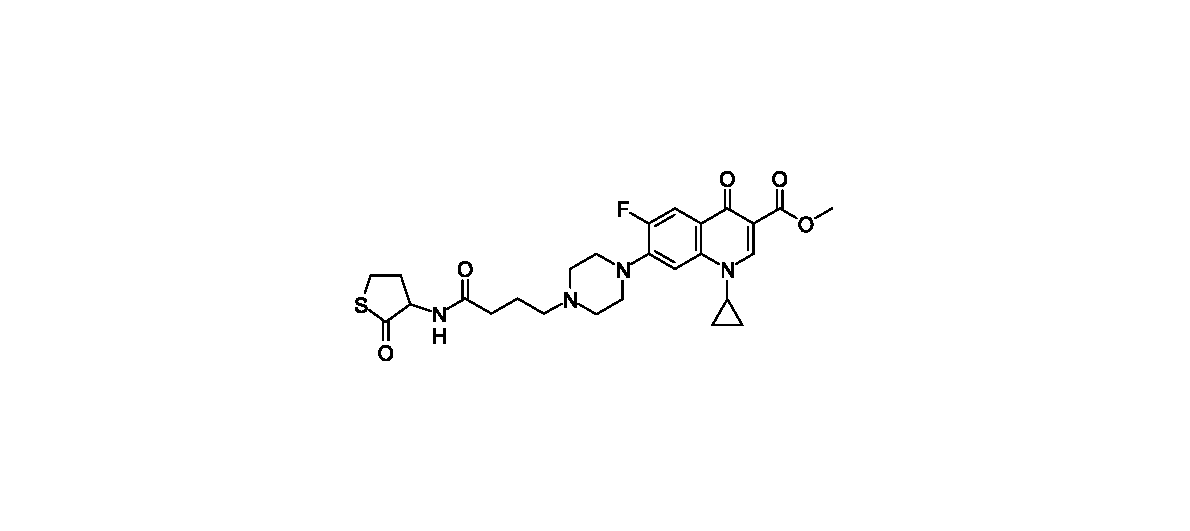
\includegraphics[scale=1]{SHL4CipMe}
		\caption{\label{fig:SHL4CipMe}}
	\end{center}
\end{figure}

\subsection{Library design}

Discuss which AHL analogues were picked + why.
Might as well make other enan of HOcy5

\begin{figure}[H]
	\begin{center}
		\schemeref[AHL]{cmpd:HL4}
		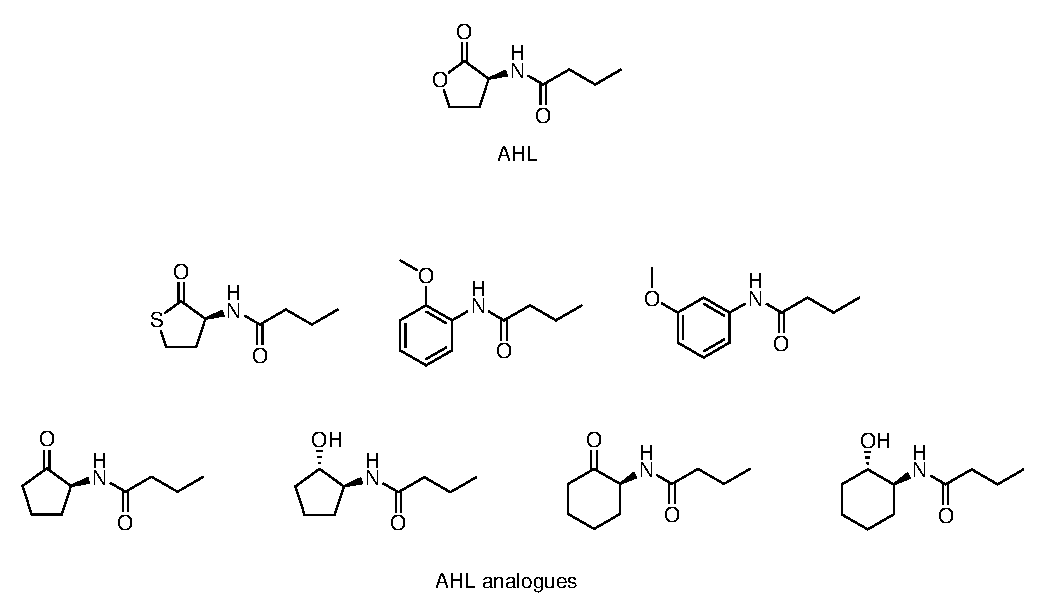
\includegraphics[scale=1]{AHL_analogues}
		\caption{\label{fig:HL4_anas}}
	\end{center}
\end{figure}

Introduce initial strategy of making bromide then azide, and diverting down the two different paths to make directly linked or triazole linked products.



%\subsubsection{Amine-linked autoinducer analogue-antibiotic conjugates}

%\subsubsection{Triazole-linked autoinducer analogue-antibiotic conjugates}

\subsection{Synthesis of the C$_4$-homocysteine thiolactone derivatives}

Methyl ciprofloxacin \compound{cmpd:CipMe} was synthesised from ciprofloxacin \compound{cmpd:Cip} and MeOH in very good yield using \textit{para}-toluenesulfonic acid as a catalyst \cite{Sachin2010}.

\begin{scheme}[H]
	\begin{center}
		\schemeref[Cip]{cmpd:Cip}	
		\schemeref[CipMe]{cmpd:CipMe}
		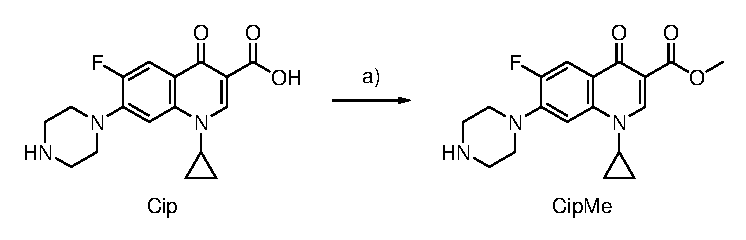
\includegraphics[scale=1]{CipMe_synth}
		\caption{a) \textit{p}-TSA, MeOH, 72 h, reflux, 83.3 \%. \label{sch:CipMe_synth}}
	\end{center}
\end{scheme}

Br-C$_4$-HCTL \compound{cmpd:SHL4Br} was synthesised using the Schotten-Baumann conditions employed previously for the Br-C$_n$-HSL compounds \compound{cmpd:HL2Br}, \compound{cmpd:HL4Br} and \compound{cmpd:HL6Br}. Br-C$_4$-HCTL \compound{cmpd:SHL4Br} was isolated in markedly higher yield than that achieved by Ganguly \textit{et al.} (87.9 \% vs. 25.0 \%). It is possible that this was due to \ce{CH2Cl2} being used for the extraction, whereas Ganguly \textit{et al.} used EtOAc.

\begin{scheme}[H]
	\begin{center}
		\schemeref[Cl4Br]{cmpd:Cl4Br}
		\schemeref[SHLHCl]{cmpd:SHLHCl}	
		\schemeref[SHL4Br]{cmpd:SHL4Br}
		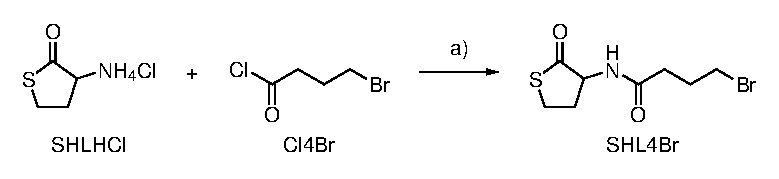
\includegraphics[scale=1]{SHL4Br_synth}
		\caption{a) \ce{NaHCO3}, \ce{CH2Cl2}, \ce{H2O}, 0 $^{\circ}$C, 1 h, 87.9 \%.\label{sch:SHL4Br_synth}}
	\end{center}
\end{scheme}

\compound{cmpd:SHL4CipMe} was synthesised using the procedure outlined by Ganguly \textit{et al.}. They don't quote a yield. Mine wasn't good.
Pig to purify. Column x2 and prep?
Got enough, not repeated.
Suggest better synth.

azide

click - just Y4Tri for now.

\todo{Eddy's, if including rest}

\begin{scheme}[H]
	\begin{center}
		\schemeref[SHL4Br]{cmpd:SHL4Br}
		\schemeref[CipMe]{cmpd:CipMe}
		\schemeref[SHL4CipMe]{cmpd:SHL4CipMe}
		\schemeref[SHL4N3]{cmpd:SHL4N3}
		\schemeref[Y4Cip]{cmpd:Y4Cip}
		\schemeref[Y4OHOCip]{cmpd:Y4OHOCip}
		\schemeref[SHL4T4Cip]{cmpd:SHL4T4Cip}
		\schemeref[SHL4THCip]{cmpd:SHL4THCip}
		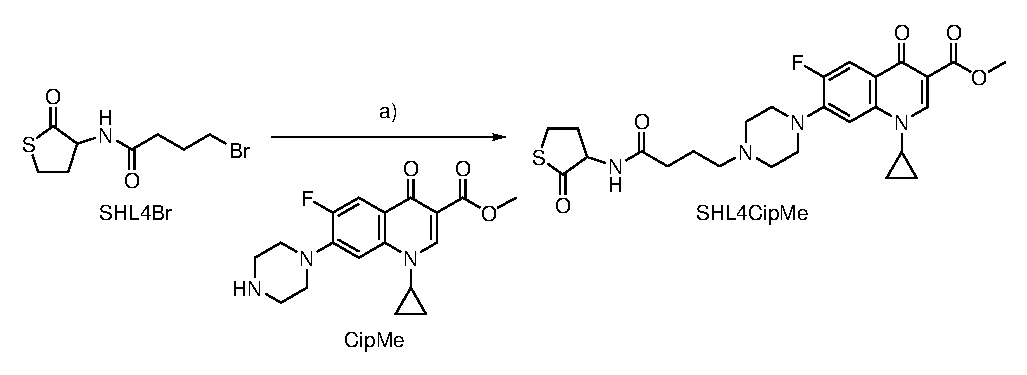
\includegraphics[scale=1]{SHL4CipMe_synth}
		\caption{
			a) \ce{K2CO3}, acetonitrile, reflux, 24 h, 12.2 \%.
			b) \ce{NaN3}, acetonitrile, 80 $^{\circ}$C, 1.5 h, 89.3 \%.
			c) \ce{CuSO4}, THPTA, sodium ascorbate, \ce{H2O}, \textit{t}-BuOH, DMSO, r.t., 7 d, 70.6 \%.\label{sch:SHL4CipMe_synth}}
	\end{center}
\end{scheme}

\todo{conditions}